\documentclass[12pt]{article}
\usepackage{setspace}
\usepackage{hyperref}
\usepackage{graphicx}
\graphicspath{ {images/} }
\onehalfspacing
\parskip=2ex
\parindent=2em
\title{Evaluation of MetaEdit+ for DSM}
\author{Jui Deshpande, Sam Minns, Glen Peek}
\date{\today}
\begin{document}
\maketitle
%Optional abstract
\begin{abstract}
In software engineering, there are many approaches for handling the kind of complexities that emerge during development.  One such approach is the use of domain-specific languages within the context of model driven development.  As model driven development has become increasingly popular, new tools have emerged with the aim of allowing users to quickly, easily, and effectively create domain-specific languages.  However, these tools are still far from mainstream.  In this paper, we critique the usability of one such metacase tool, MetaEdit+, by defining a domain-specific language for a library system, describing the creation of this language using MetaEdit+, and reviewing our final result.  
\end{abstract}
\section{Introduction}
In this project we create a simple library management system in MetaEdit+. The solution consists of some basic building blocks, such as books, authors, librarians. 
\section{Language Design Background}
People find DSLs valuable because a well-designed DSL can be much easier to program with than a traditional library. This improves programmer productivity, which is always valuable. In particular it may also improve communication with domain experts, which is an important tool for tackling one of the hardest problems in software development.
\section{MetaEdit+}
With MetaEdit+ an experienced developer defines a domain specific language containing the domain’s concepts and rules in a metamodel, and specifies the mapping from that to code in a domain-specific code generator. For the modeling language implementation, MetaEdit+ provides a metamodeling tool suite for defining the language concepts, rules, symbols, checking reports and generators. Next to the user’s guide, developers are able to watch several webcasts, read articles, blogs, brochures and even listen to podcasts. Generally, Metacase provides really good and clear documentation, but some points could certainly be refined.

Documentation provided
MetaEdit+ offers various DSM resources. This includes a detailed Workbench User’s Guide which discusses every aspect of metamodeling in MetaEdit+. All methods provided by the API are described as well. A single point of criticism in the guide is the rather brief explanation of the API methods and the few examples it delivers.
\section{Library Language}
The Domain Specific Language we have created is an attempt at modelling a Library. We have a chosen the context of a public library as opposed to a specialised facility such as a university or law library. The DSL is naturally constrained by our development tool and as such  is comprised of three main entities. Objects represent physical entities such as loanable items, library equipment and people such as library users and employees. Relationships describe methods by which objects within the DSL may interact. Roles define constraints on the types of objects that may mutually INHABIT? TAKE THE PLACE IN THE RELATIONSHIP, ?BE?, ?RESIDE? word please  end of a relationship between those objects. Additionally constraints may be defined surrounding the semantics of relationships. These constraints fall into four categories:
Connectivity: cardinality and type of some shit about the thing with a thing. 
Occurrence: constraint surrounding the number of a unique objects may appear in a graph
Uniqueness: uniqueness constraints for property values such as ID etc
Port: No fucking idea what the shit port was for, probably something to do with ships.
Creating and applying constraints allows further development and enrichment of DSL semantics.  
\subsection{Objects}
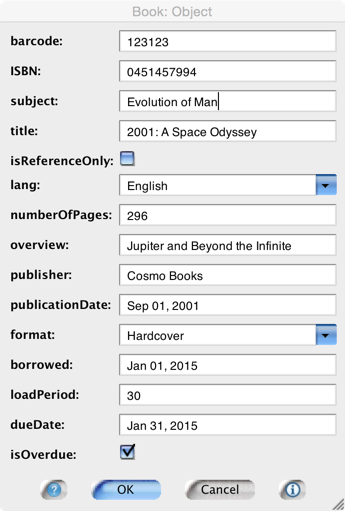
\includegraphics[width=0.5\textwidth]{obj_book}
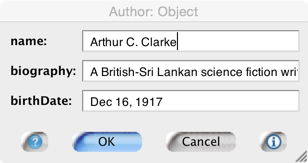
\includegraphics[width=0.5\textwidth]{obj_author}
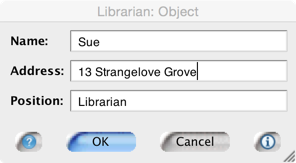
\includegraphics[width=0.5\textwidth]{obj_librarian}
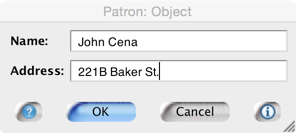
\includegraphics[width=0.5\textwidth]{obj_patron}

\subsection{Relationships/Roles}
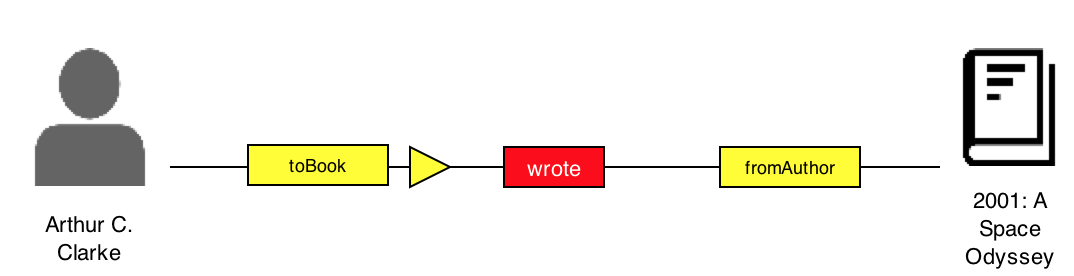
\includegraphics[width=0.5\textwidth]{rel_wrote}
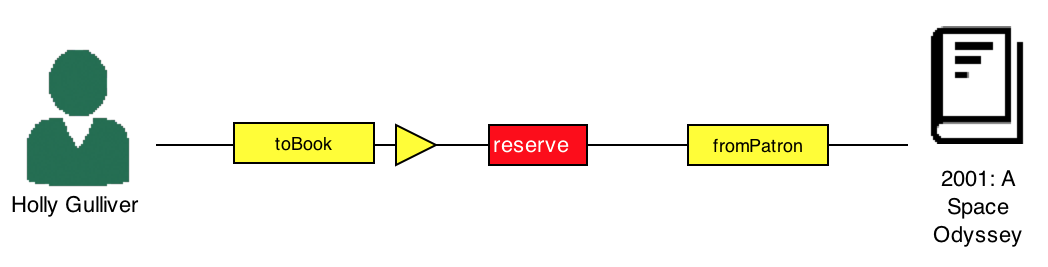
\includegraphics[width=0.5\textwidth]{rel_reserve}
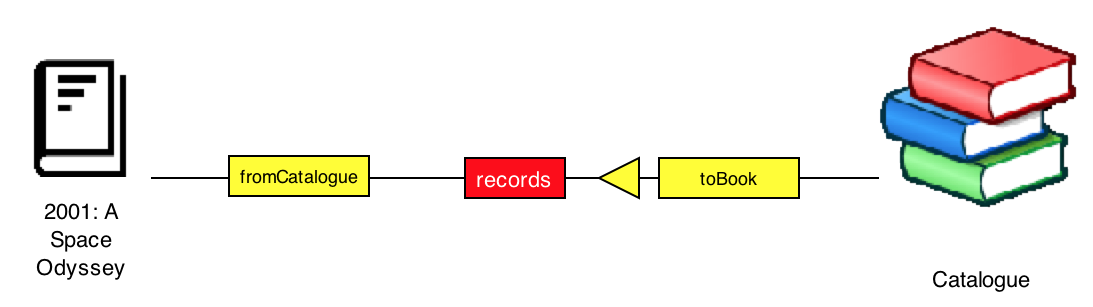
\includegraphics[width=0.5\textwidth]{rel_records}


\subsection{Abstract Syntax}
\section{Discussion about Tool}
We undertook an initial survey both of the tools recommended to us and those identified through literature review (a complete lie but saying ‘we googled it’ sucks). 
We rejected a number of tools such as GME due to platform limitations. These tools were only usable within a Windows environment which was unsuitable for our team. Other alternatives such as DOME were rejected due to no longer being maintained and thus unavailable. AtomPM was no longer being maintained and was dependent on legacy versions of NPM packages which rendered it uninstallable, unstable and unusable. Eclipse plugin tools such as Marama and XMF similarly were dependent on legacy versions of Eclipse IDE. The Marama modelling tool was ‘end of lifed’ in 2012 which had the consequence of non existent support or help resources. XMF is no longer maintained and is currently not supported in any modern version of Eclipse and while XMF will load, it no longer functions in any usable way. 
Other tools are available, however, the majority require a licence to be purchased in order to access any meaningful functionality. With these factors in mind we selected to use the only remaining option which was MetaEdit+.
\subsection{Evaluation Version}
In using MetaEdit+ we encountered a number of limitations that complicated our development processes. Specifically the limited functionality available through the evaluation license significantly reduced our efficiency as a team. In order to work effectively as a group a concurrent working environment is imperative. In MetaEdit+ team collaboration functionality is limited to paid licenses. In an effort to circumvent this limitation we attempted to implement a GIT workflow, however, as the files used by MetaEdit+ to maintain a project are binaries this was unsuccessful. Had we been able to work concurrently and collaboratively our workflow would have been considerably smoother and more productive. MetaEdit+ uses a kind of version control workflow internally, using the concept of repositories and commits to manage the development of a model. Had we been able to take advantage of this the learning and prototyping phase might have yielded more in the way of usable artifacts. As it transpired the majority of our learning and prototyping artifacts were unusable as the merging of projects was something our licence did not allow.


\bibliographystyle{acm}
\bibliography{mybib}
\end{document}